\documentclass{ximera}
%% You can put user macros here
%% However, you cannot make new environments

\listfiles

\graphicspath{{./}{firstExample/}{secondExample/}}

\usepackage{tikz}
\usepackage{tkz-euclide}
\usepackage{tikz-3dplot}
\usepackage{tikz-cd}
\usetikzlibrary{shapes.geometric}
\usetikzlibrary{arrows}
%\usetkzobj{all}
\pgfplotsset{compat=1.13} % prevents compile error.

%\renewcommand{\vec}[1]{\mathbf{#1}}
\renewcommand{\vec}{\mathbf}
\newcommand{\RR}{\mathbb{R}}
\newcommand{\dfn}{\textit}
\newcommand{\dotp}{\cdot}
\newcommand{\id}{\text{id}}
\newcommand\norm[1]{\left\lVert#1\right\rVert}
 
\newtheorem{general}{Generalization}
\newtheorem{initprob}{Exploration Problem}

\tikzstyle geometryDiagrams=[ultra thick,color=blue!50!black]

%\DefineVerbatimEnvironment{octave}{Verbatim}{numbers=left,frame=lines,label=Octave,labelposition=topline}



\usepackage{mathtools}


\title{Application to Electrical Networks} \license{CC BY-NC-SA 4.0}

\begin{document}

\begin{abstract}
 \end{abstract}
\maketitle

\begin{onlineOnly}
\section*{Application to Electrical Networks}
\end{onlineOnly}

In an electrical network it is often necessary to find the current in amperes ($A$) flowing in various parts of the network. These networks usually contain resistors that retard the current. Resistance is measured in ohms ($\Omega$). The current is increased at various points by voltage sources (for example, a battery). The voltage of these sources is measured in volts (V). We use the following symbols to represent resistors and voltage sources:
\begin{image}
   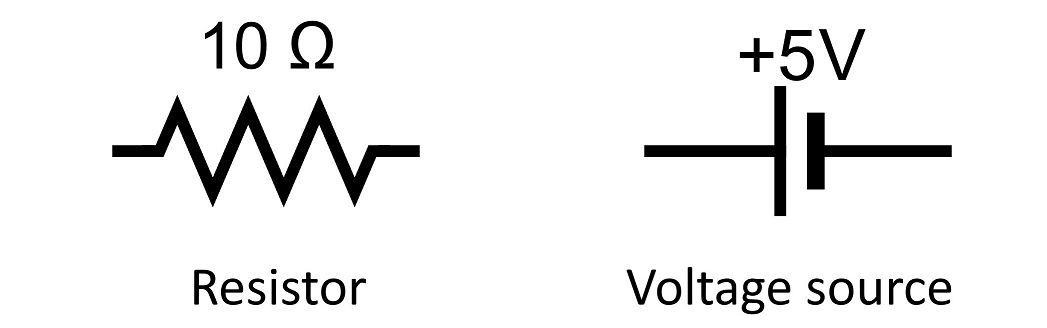
\includegraphics[height=0.25in]{circuit7.jpg}~
 \end{image}

We assume these voltage sources have no resistance. The flow of current is governed by the following principles.

\begin{theorem}[Ohm's Law]\label{001806}

The current $I$ and the voltage drop $V$ across a resistance $R$ are related by the equation $V = RI$.\index{Ohm's Law}

\end{theorem}

\begin{theorem}[Kirchhoff's Laws]\label{001809}
    Each of the following is true in an electric circuit.
\begin{enumerate}
    \item\label{item:001809j}(Junction Rule) The current flow into a junction equals the current flow out of that junction.
    \item\label{item:001809c}(Circuit Rule) The algebraic sum of the voltage drops (due to resistances) around any closed circuit of the network must equal the sum of the voltage increases around the circuit.
\end{enumerate}

\end{theorem}

When applying the Circuit Rule, select a direction (clockwise or counterclockwise) around the closed circuit and then consider all voltages and currents positive when in this direction
and negative when in the opposite direction. %This is why the term \textit{algebraic sum} is used in rule 2. 
Here is an example.

\begin{example}\label{001817}

Find the various currents in the circuit shown.

\begin{image}
   
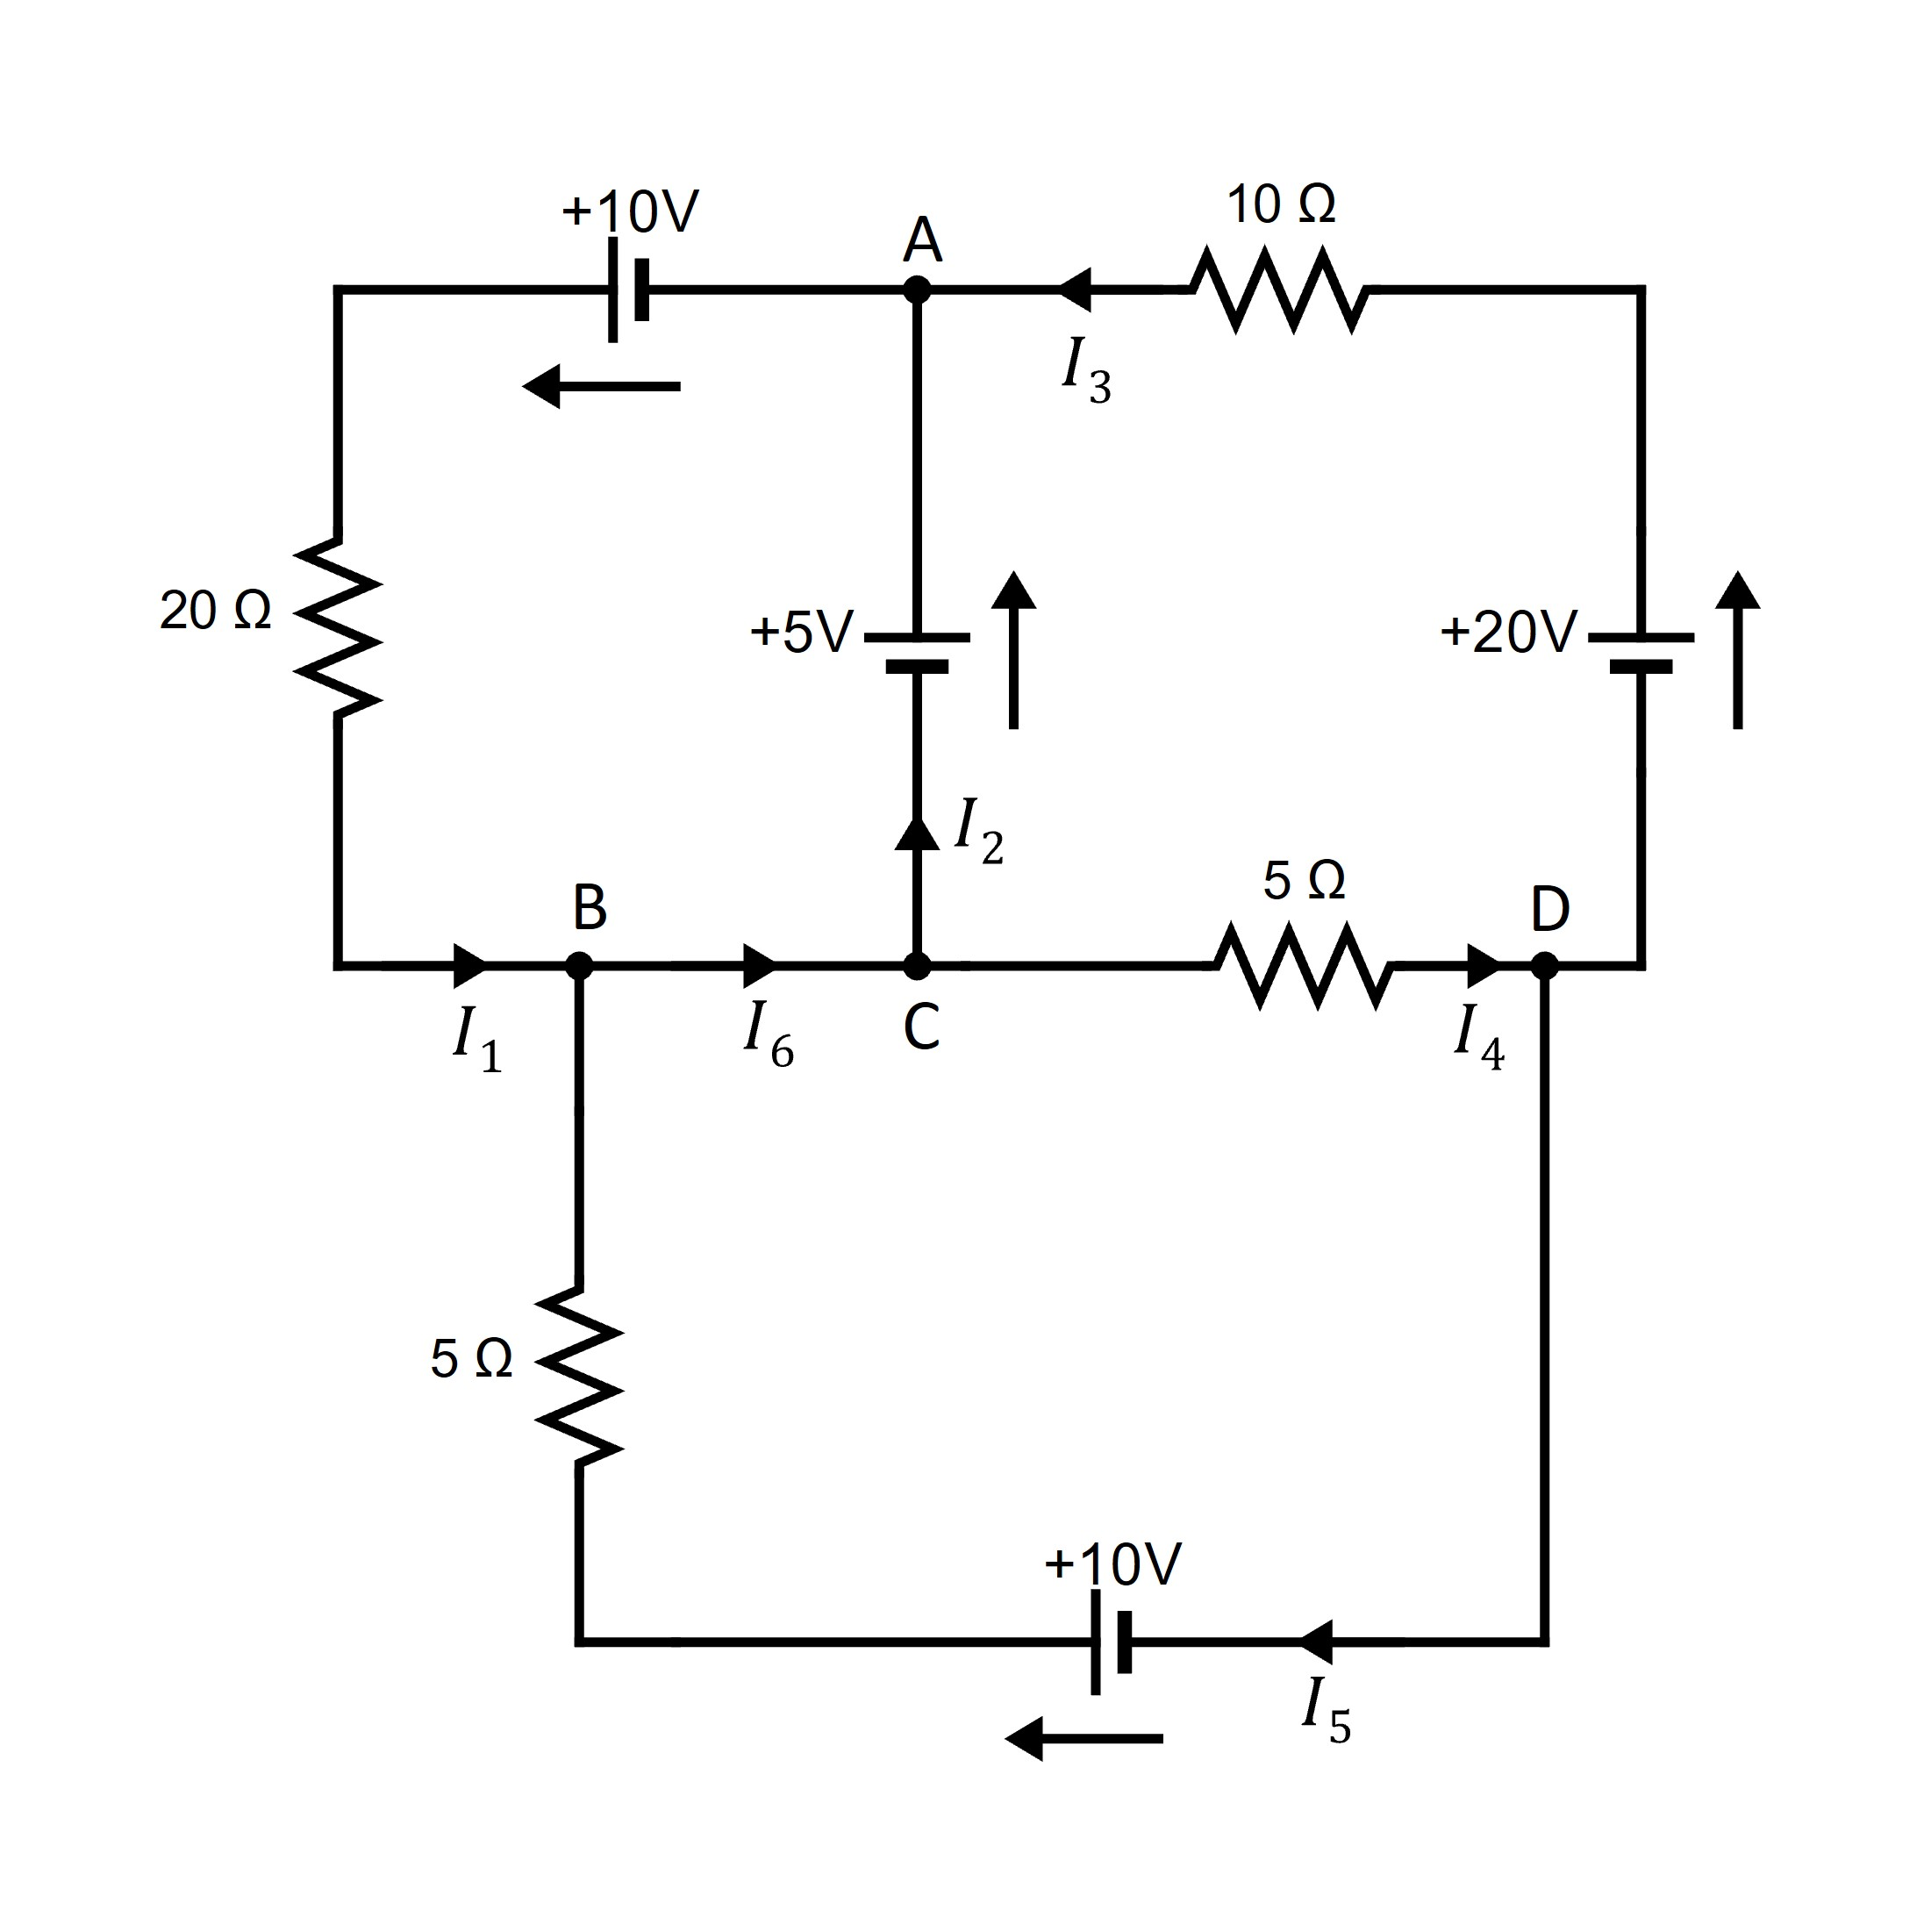
\includegraphics[height=1.5in]{circuit100.jpg}~
 
\end{image}

\begin{explanation}
  First apply the junction rule at junctions $A$, $B$, $C$, and $D$ to obtain


$$\begin{array}{lccccccc}
	\mbox{Junction } A:\quad &&& I_1 & = & I_2 &+& I_3 \\
	\mbox{Junction } B:\quad &&& I_6 & = & I_1 &+& I_5 \\
	\mbox{Junction } C:\quad & I_2 &+& I_4 & = & I_6 && \\
	\mbox{Junction } D:\quad & I_3 &+& I_5 & = & I_4&& \\
\end{array}$$

Note that these equations are not independent (in fact, the third is an easy consequence of the other three).

Next, the circuit rule insists that the sum of the voltage increases (due to the sources) around a closed circuit must equal the sum of the voltage drops (due to resistances). By Ohm's law, the voltage loss across a resistance $R$ (in the direction of the current $I$) is $RI$. Going counterclockwise around three closed circuits yields

$$\begin{array}{lcccccccc}
	\mbox{Upper left: } \quad\quad  &10 & + & 5 & = & 20I_1 && \\
	\mbox{Upper right: } &-5 & +& 20 & = & 10I_3& +& 5I_4 \\
	\mbox{Lower: } && &-10 & = & -5I_5 &-& 5I_4 \\
\end{array}$$

Hence, disregarding the redundant equation obtained at junction $C$, we have six equations in the six unknowns $I_1, \dots, I_6$. The solution is

$$\begin{array}{ccccccc}
I_1& =& \frac{15}{20}&\quad& I_2 &=& \frac{-1}{20}\\
&&&&&&\\
I_3& =& \frac{16}{20}&\quad& I_4 &=& \frac{28}{20}\\
&&&&&&\\
I_5 &=& \frac{12}{20}&\quad&I_6 &=& \frac{27}{20}
\end{array}$$

The fact that $I_2$ is negative means, of course, that this current is in the opposite direction, with a magnitude of $\frac{1}{20}$ amperes.

\end{explanation}

\end{example}

\section*{Practice Problems}

In Exercises 1 to 4, find the currents in the circuits.

\begin{problem}\label{prob:circuit1}
\begin{image}
   
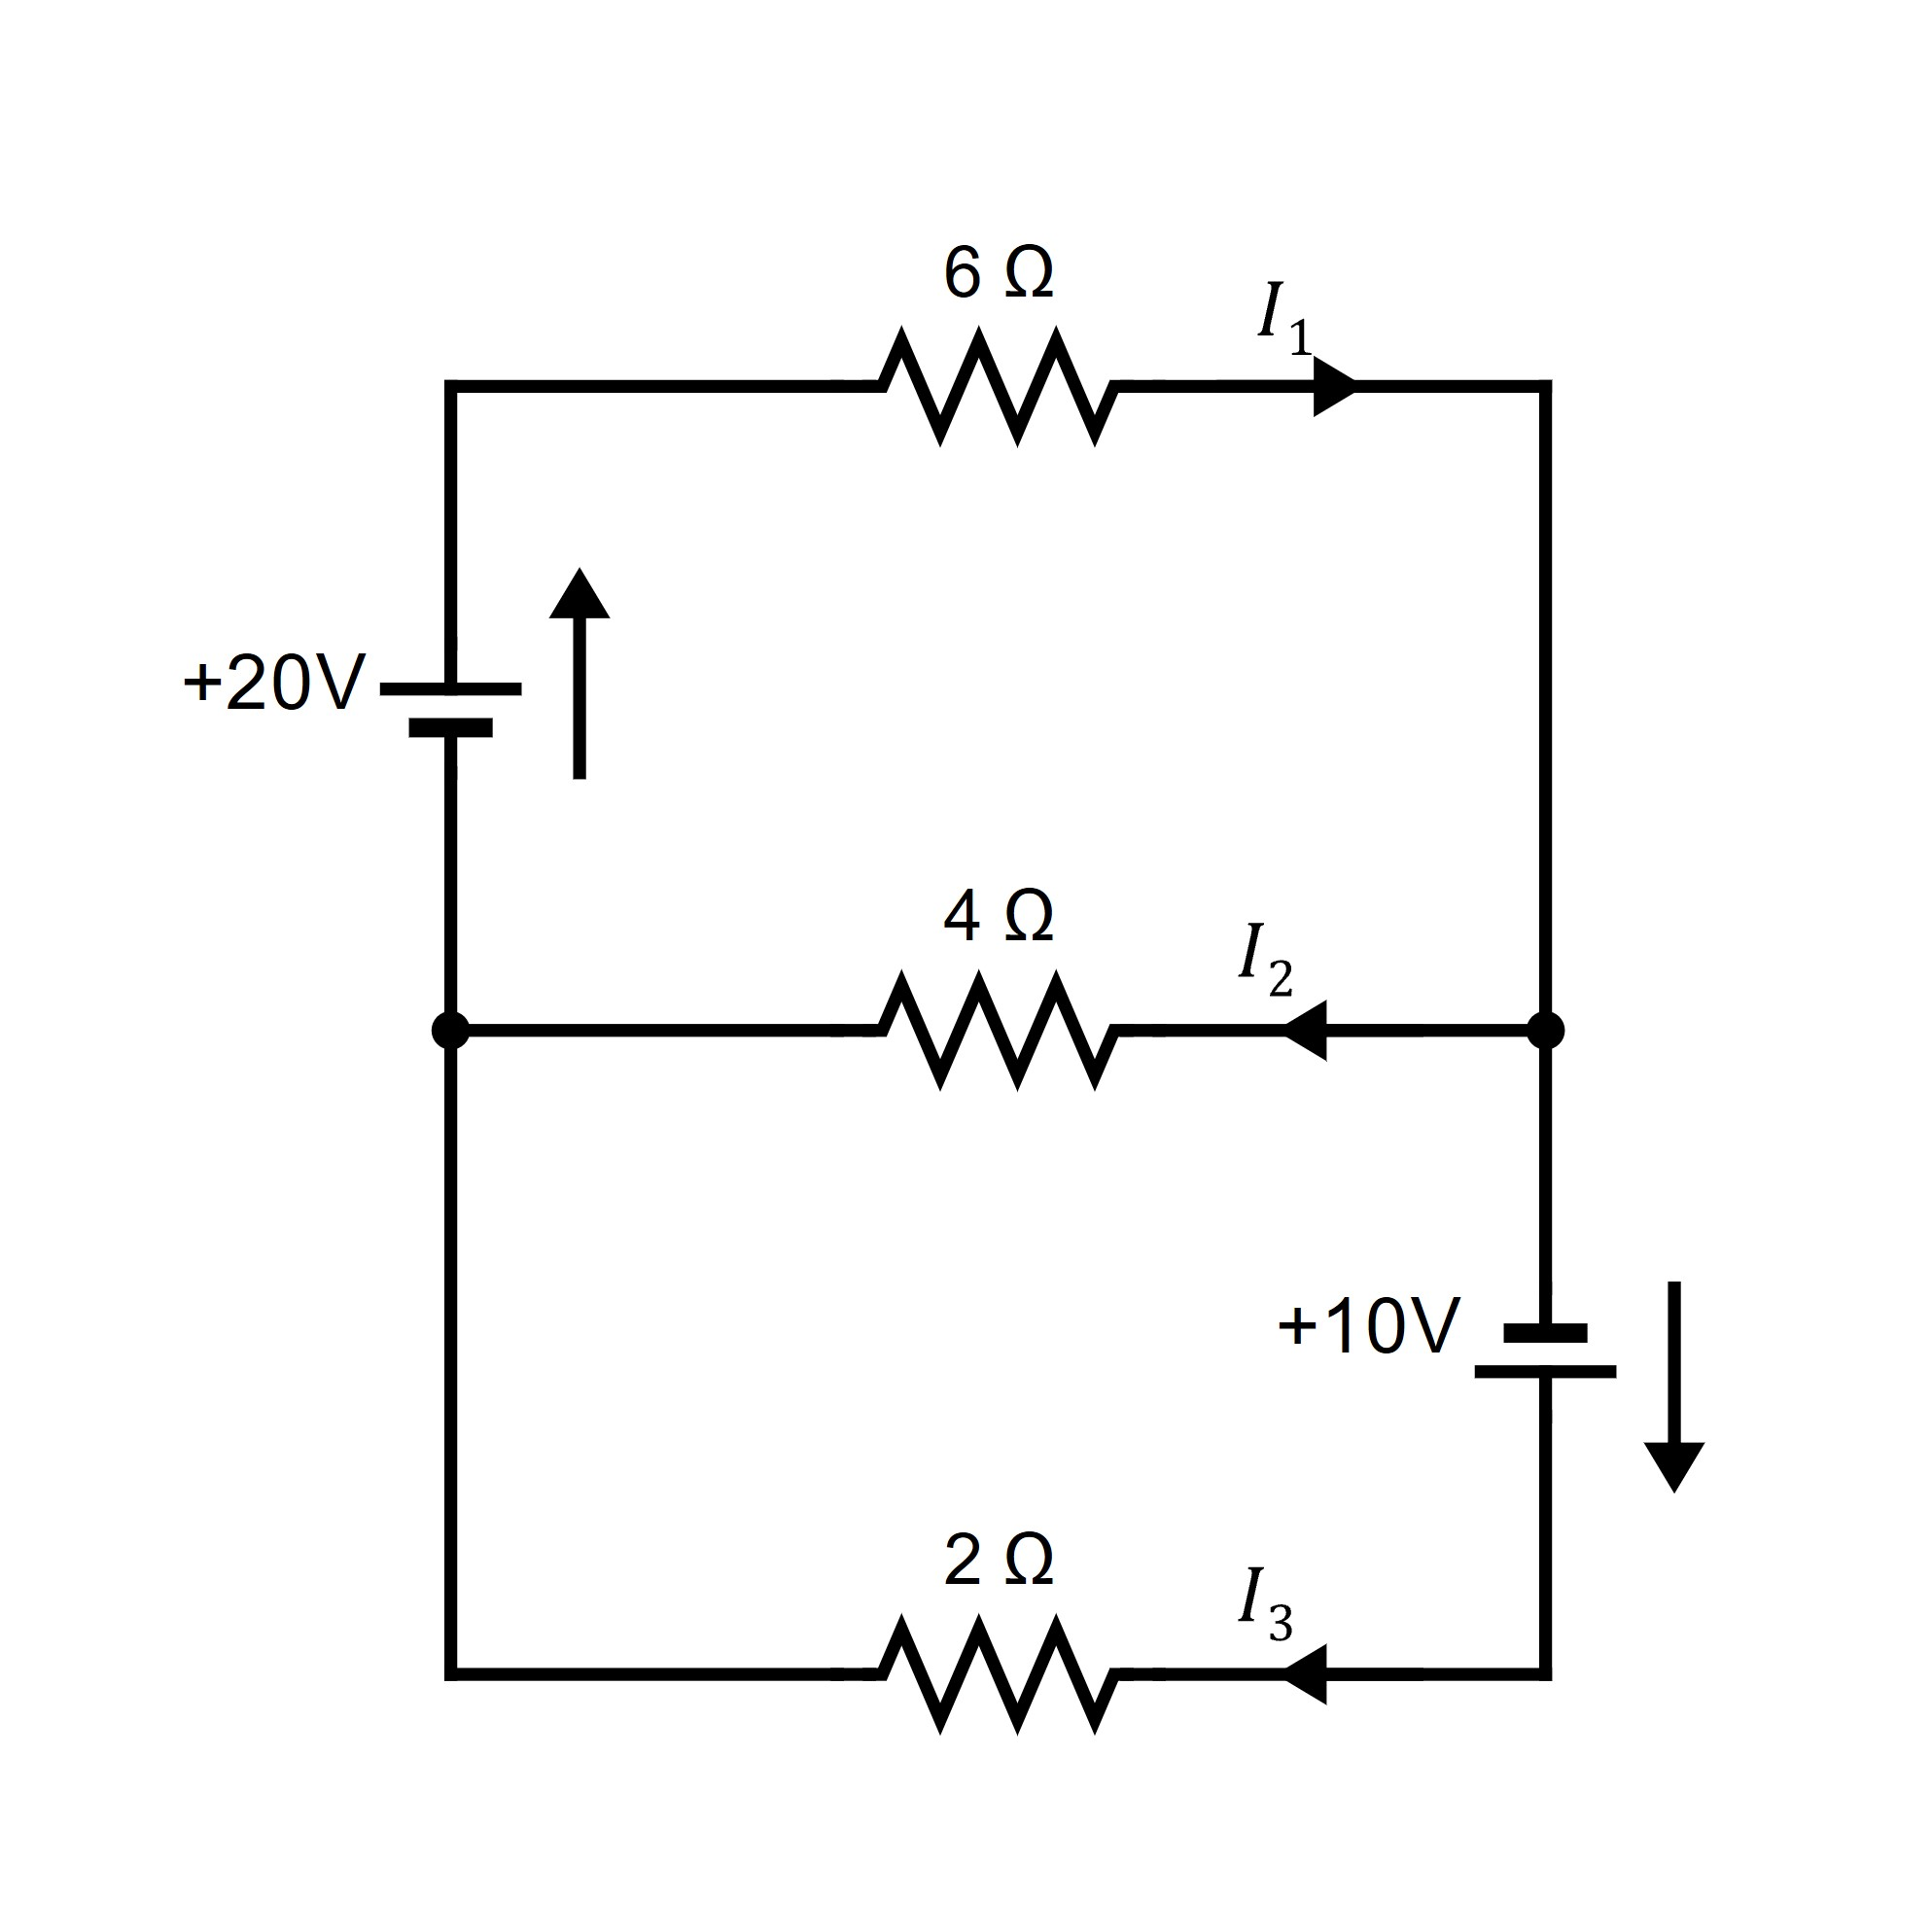
\includegraphics[height=1.2in]{circuit200.jpg}~
 
\end{image}

$ I_1 = \answer{\frac{40}{11}}$, $I_2 = \answer{-\frac{5}{11}}$, $I_3 = \answer{\frac{45}{11}}$

\end{problem}

\begin{problem}\label{prob:circuit2}

\begin{image}
   
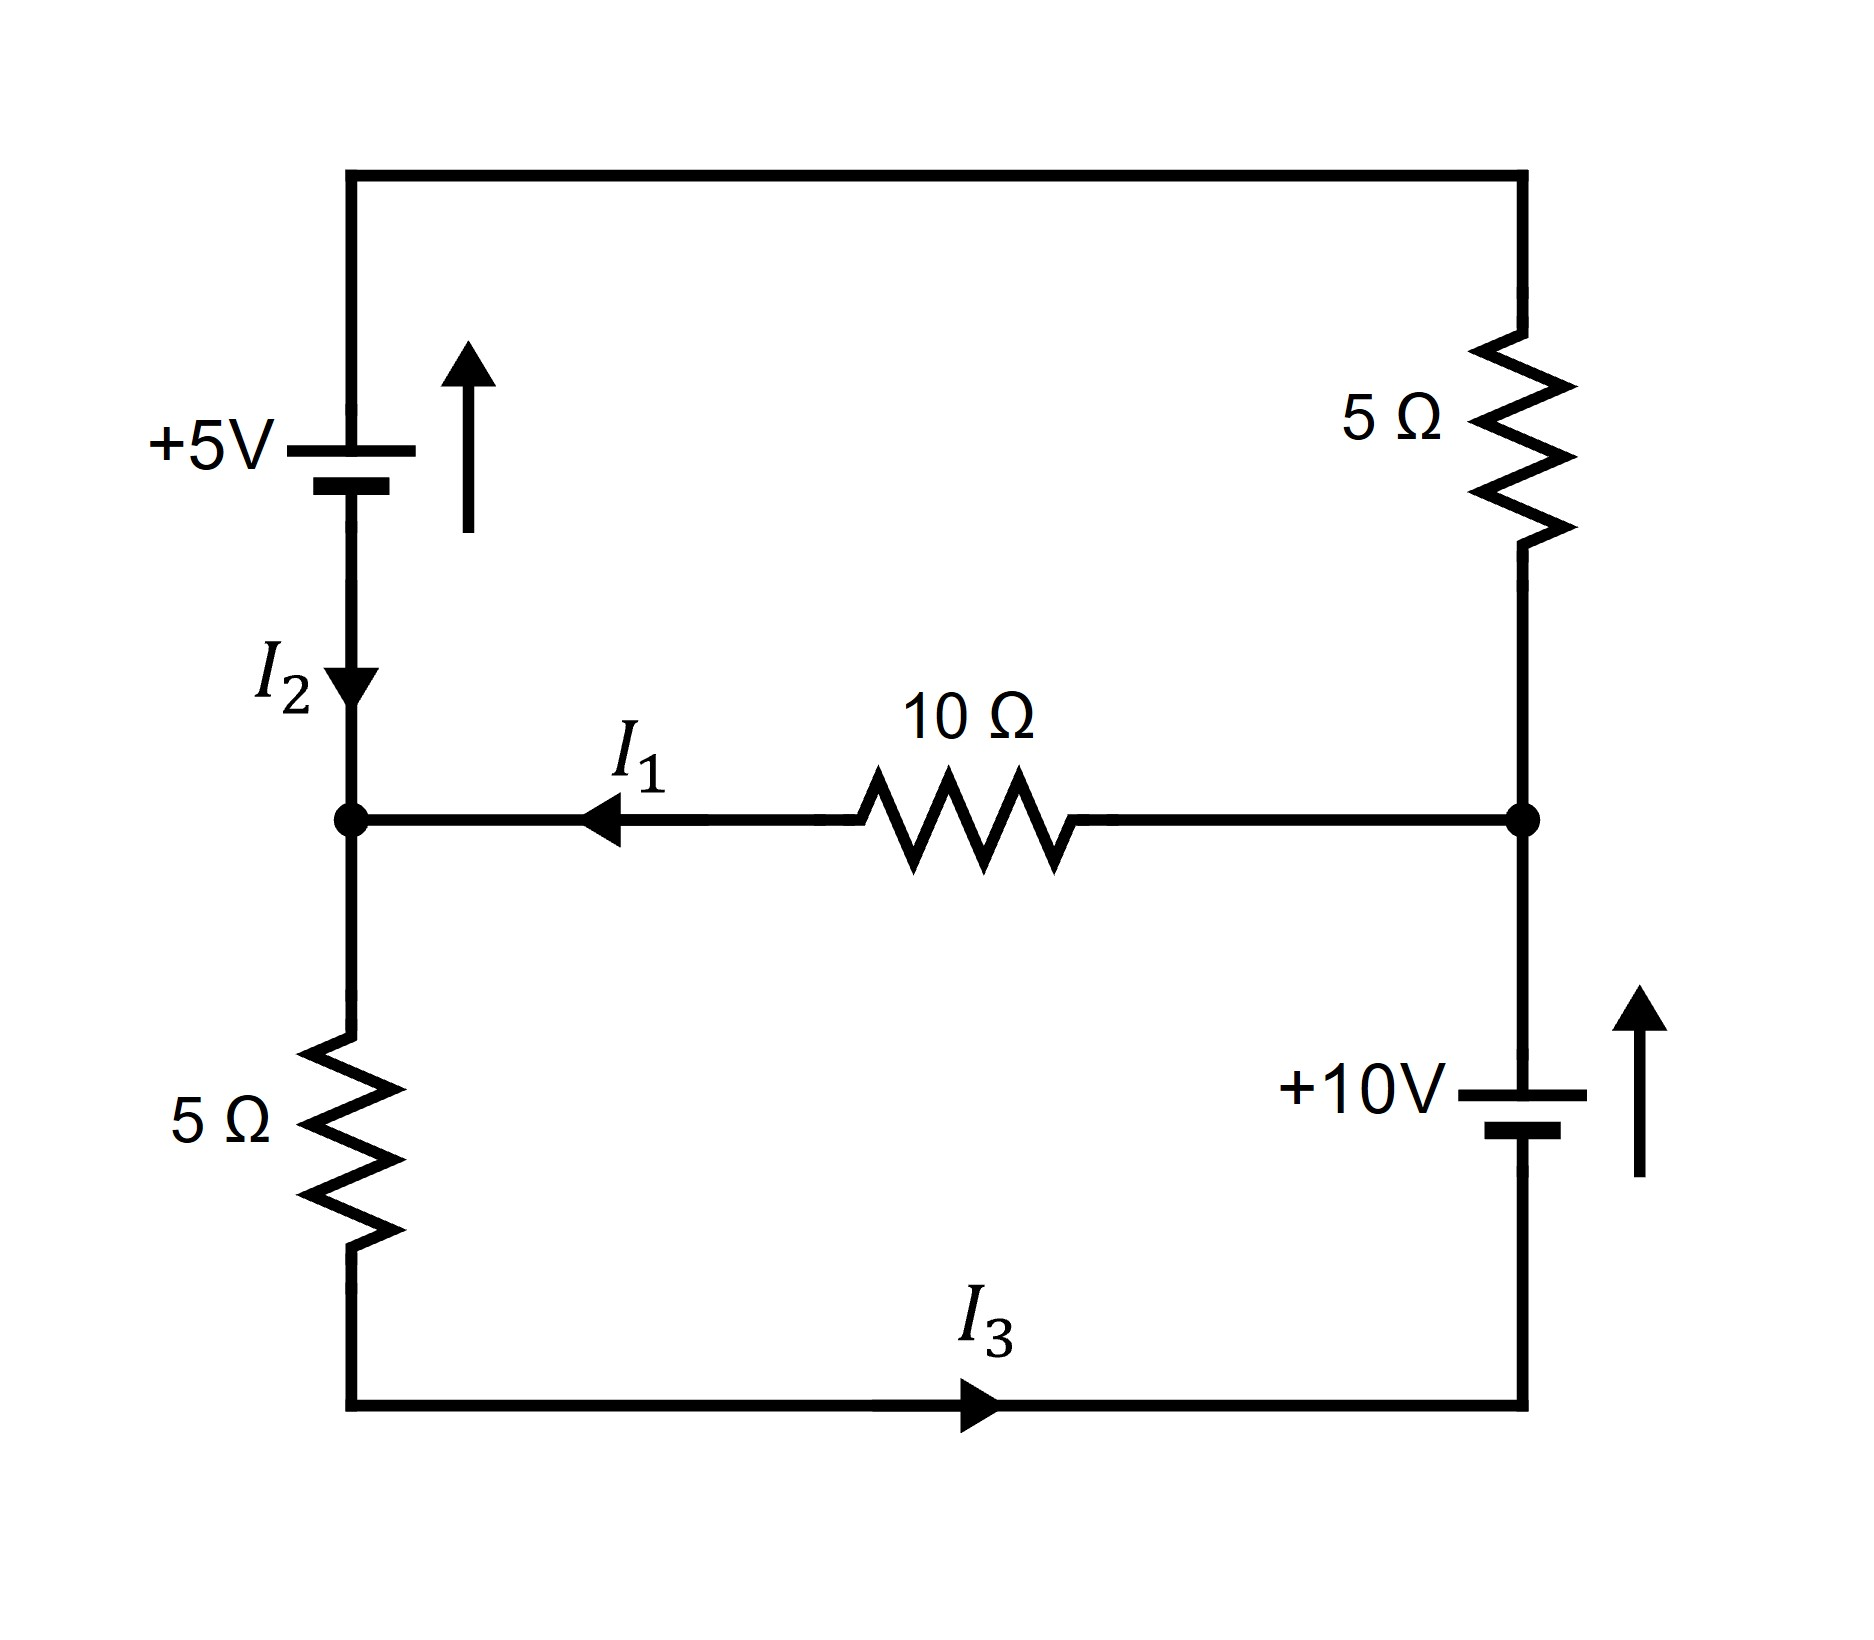
\includegraphics[height=1in]{circuit300.jpg}~
 
\end{image}

%$ I_1 = \answer{-\frac{1}{5}}$, $I_2 = \answer{\frac{3}{5}}$, $I_3 = \answer{\frac{4}{5}}$

$ I_1 = \answer{\frac{3}{5}}$, $I_2 = \answer{-\frac{1}{5}}$, $I_3 = \answer{\frac{4}{5}}$


\end{problem}

\begin{problem}\label{prob:circuit4}
\begin{image}
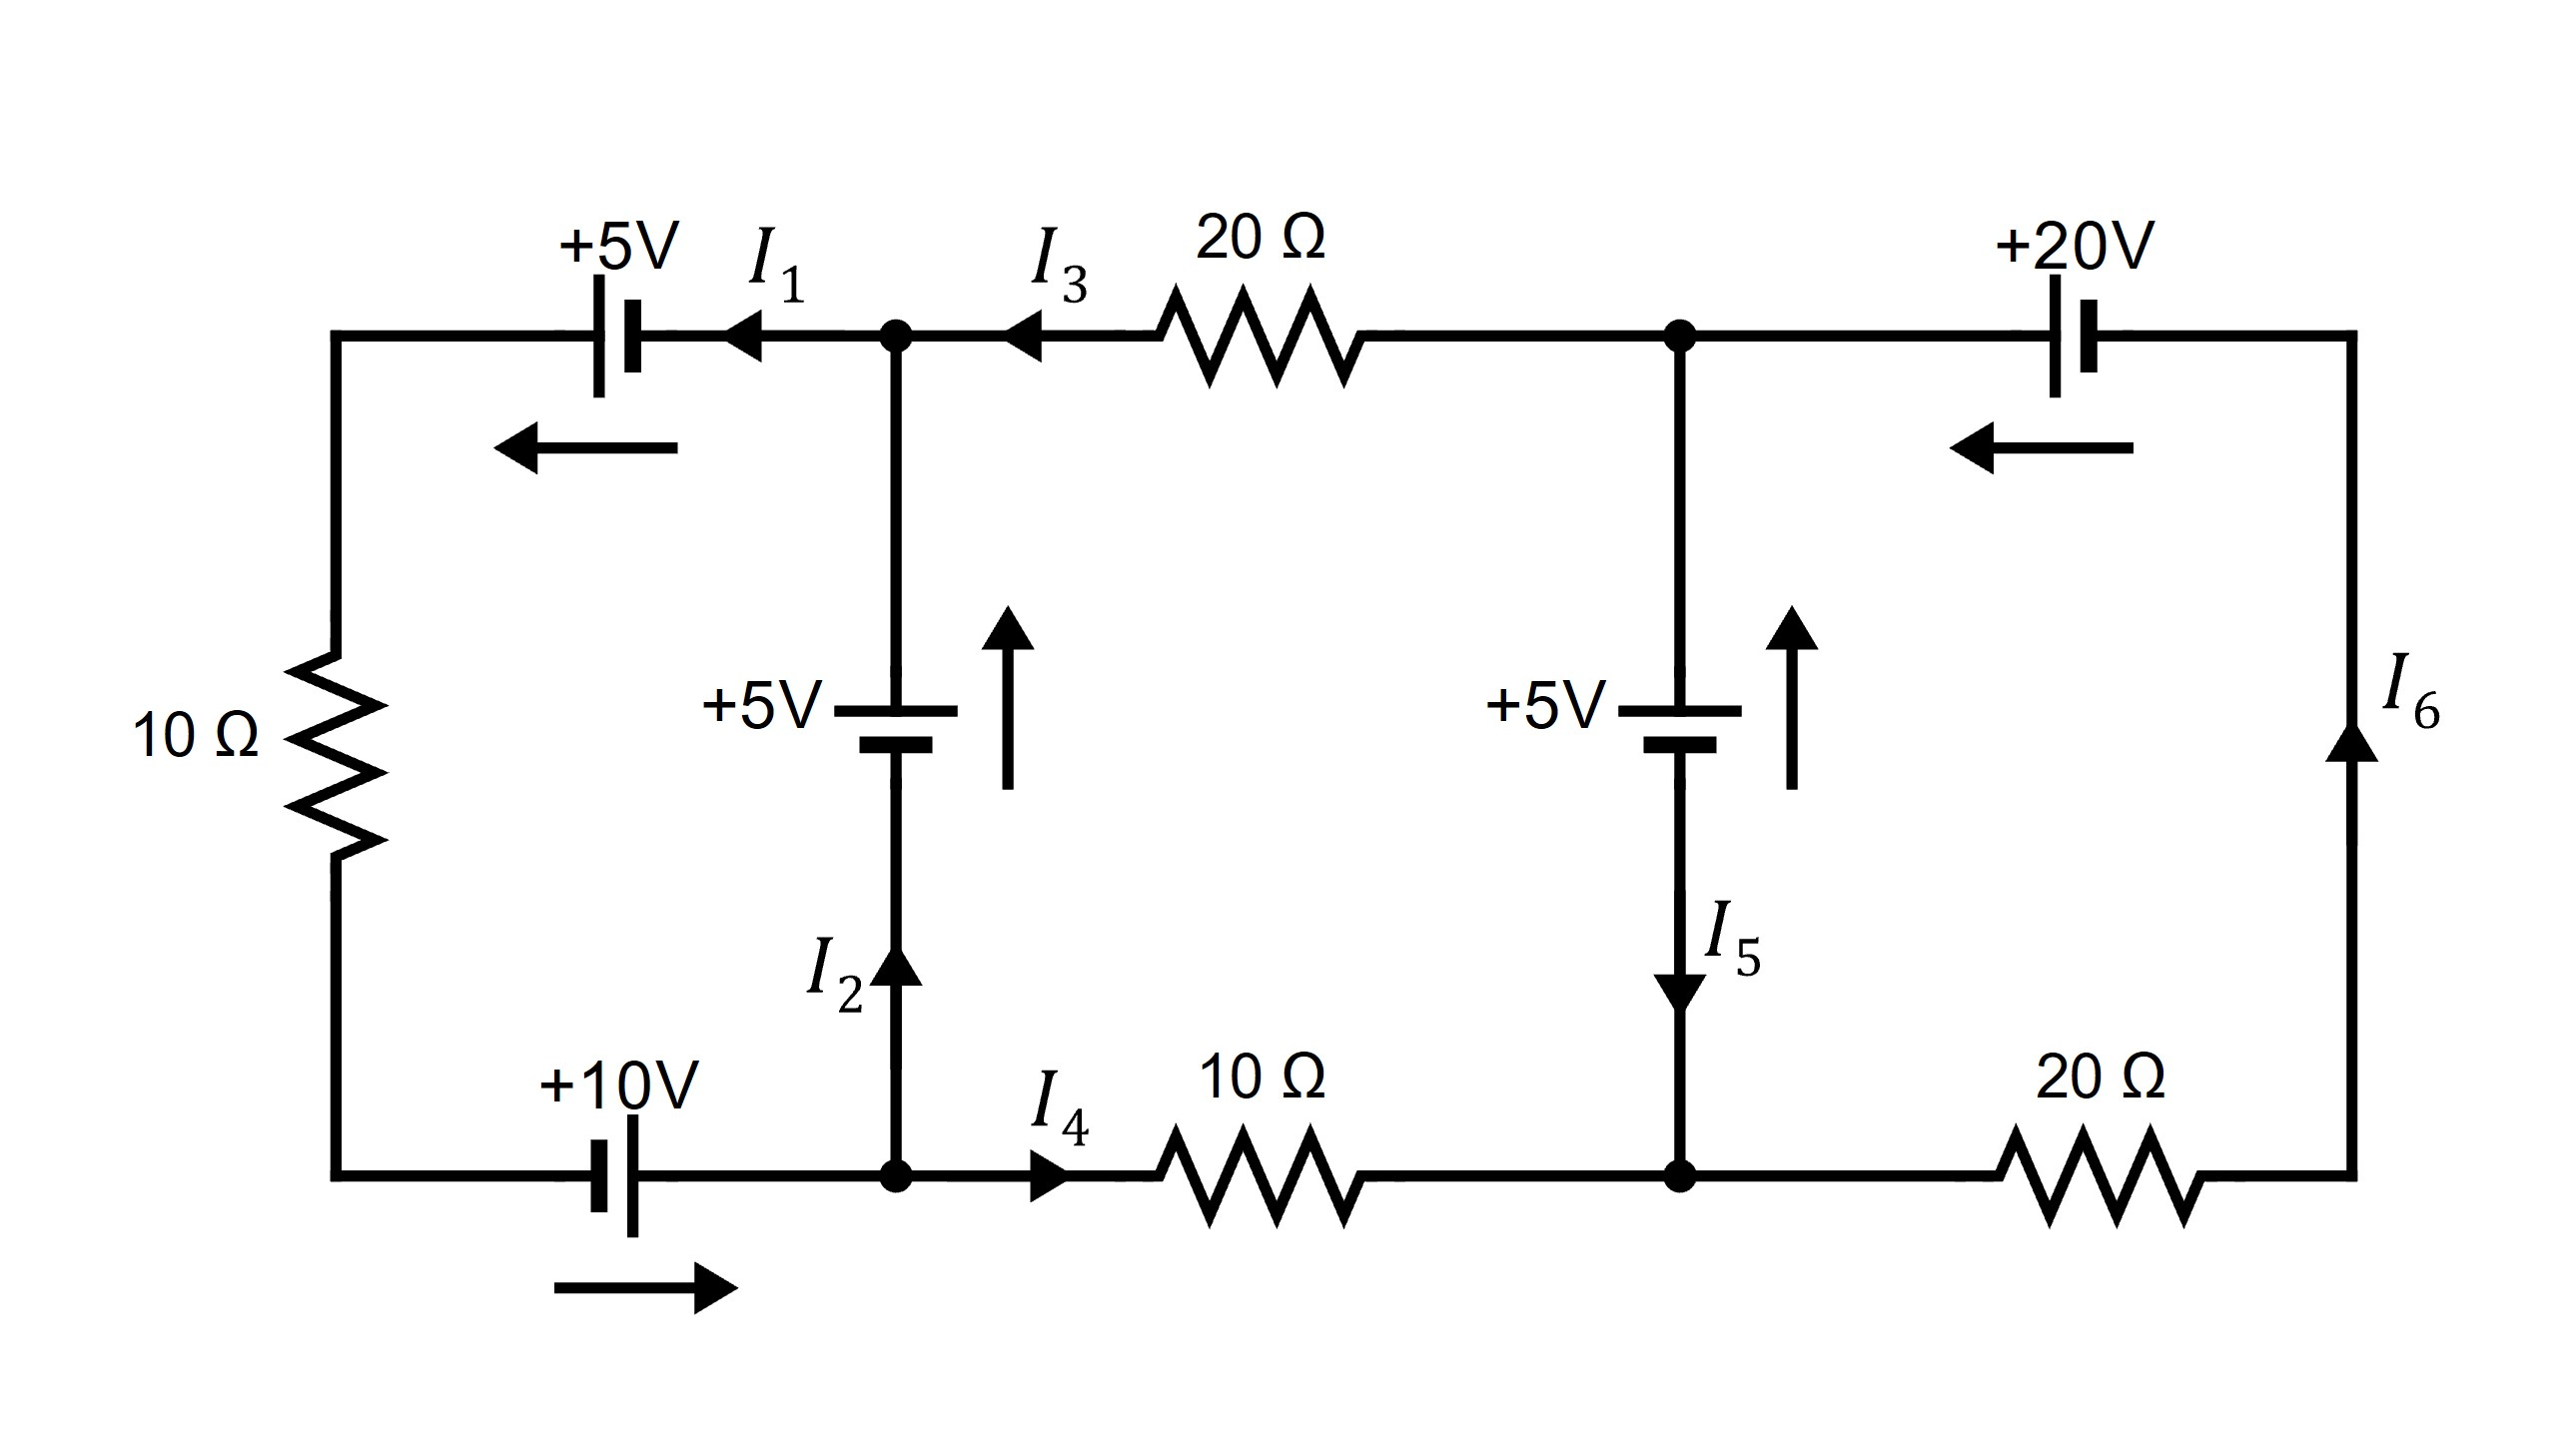
\includegraphics[height=1.2in]{circuit400.jpg}~

\end{image}

$ I_1 = \answer{2}$, $I_2 = \answer{2}$, $I_3 = \answer{0}$, $I_4 = \answer{0}$, $I_5 = \answer{\frac{3}{4}}$, $I_6 = \answer{\frac{3}{4}}$
\end{problem}

\begin{problem}\label{prob:circuit5}
%All resistances are $10 \Omega$.

\begin{image}
   
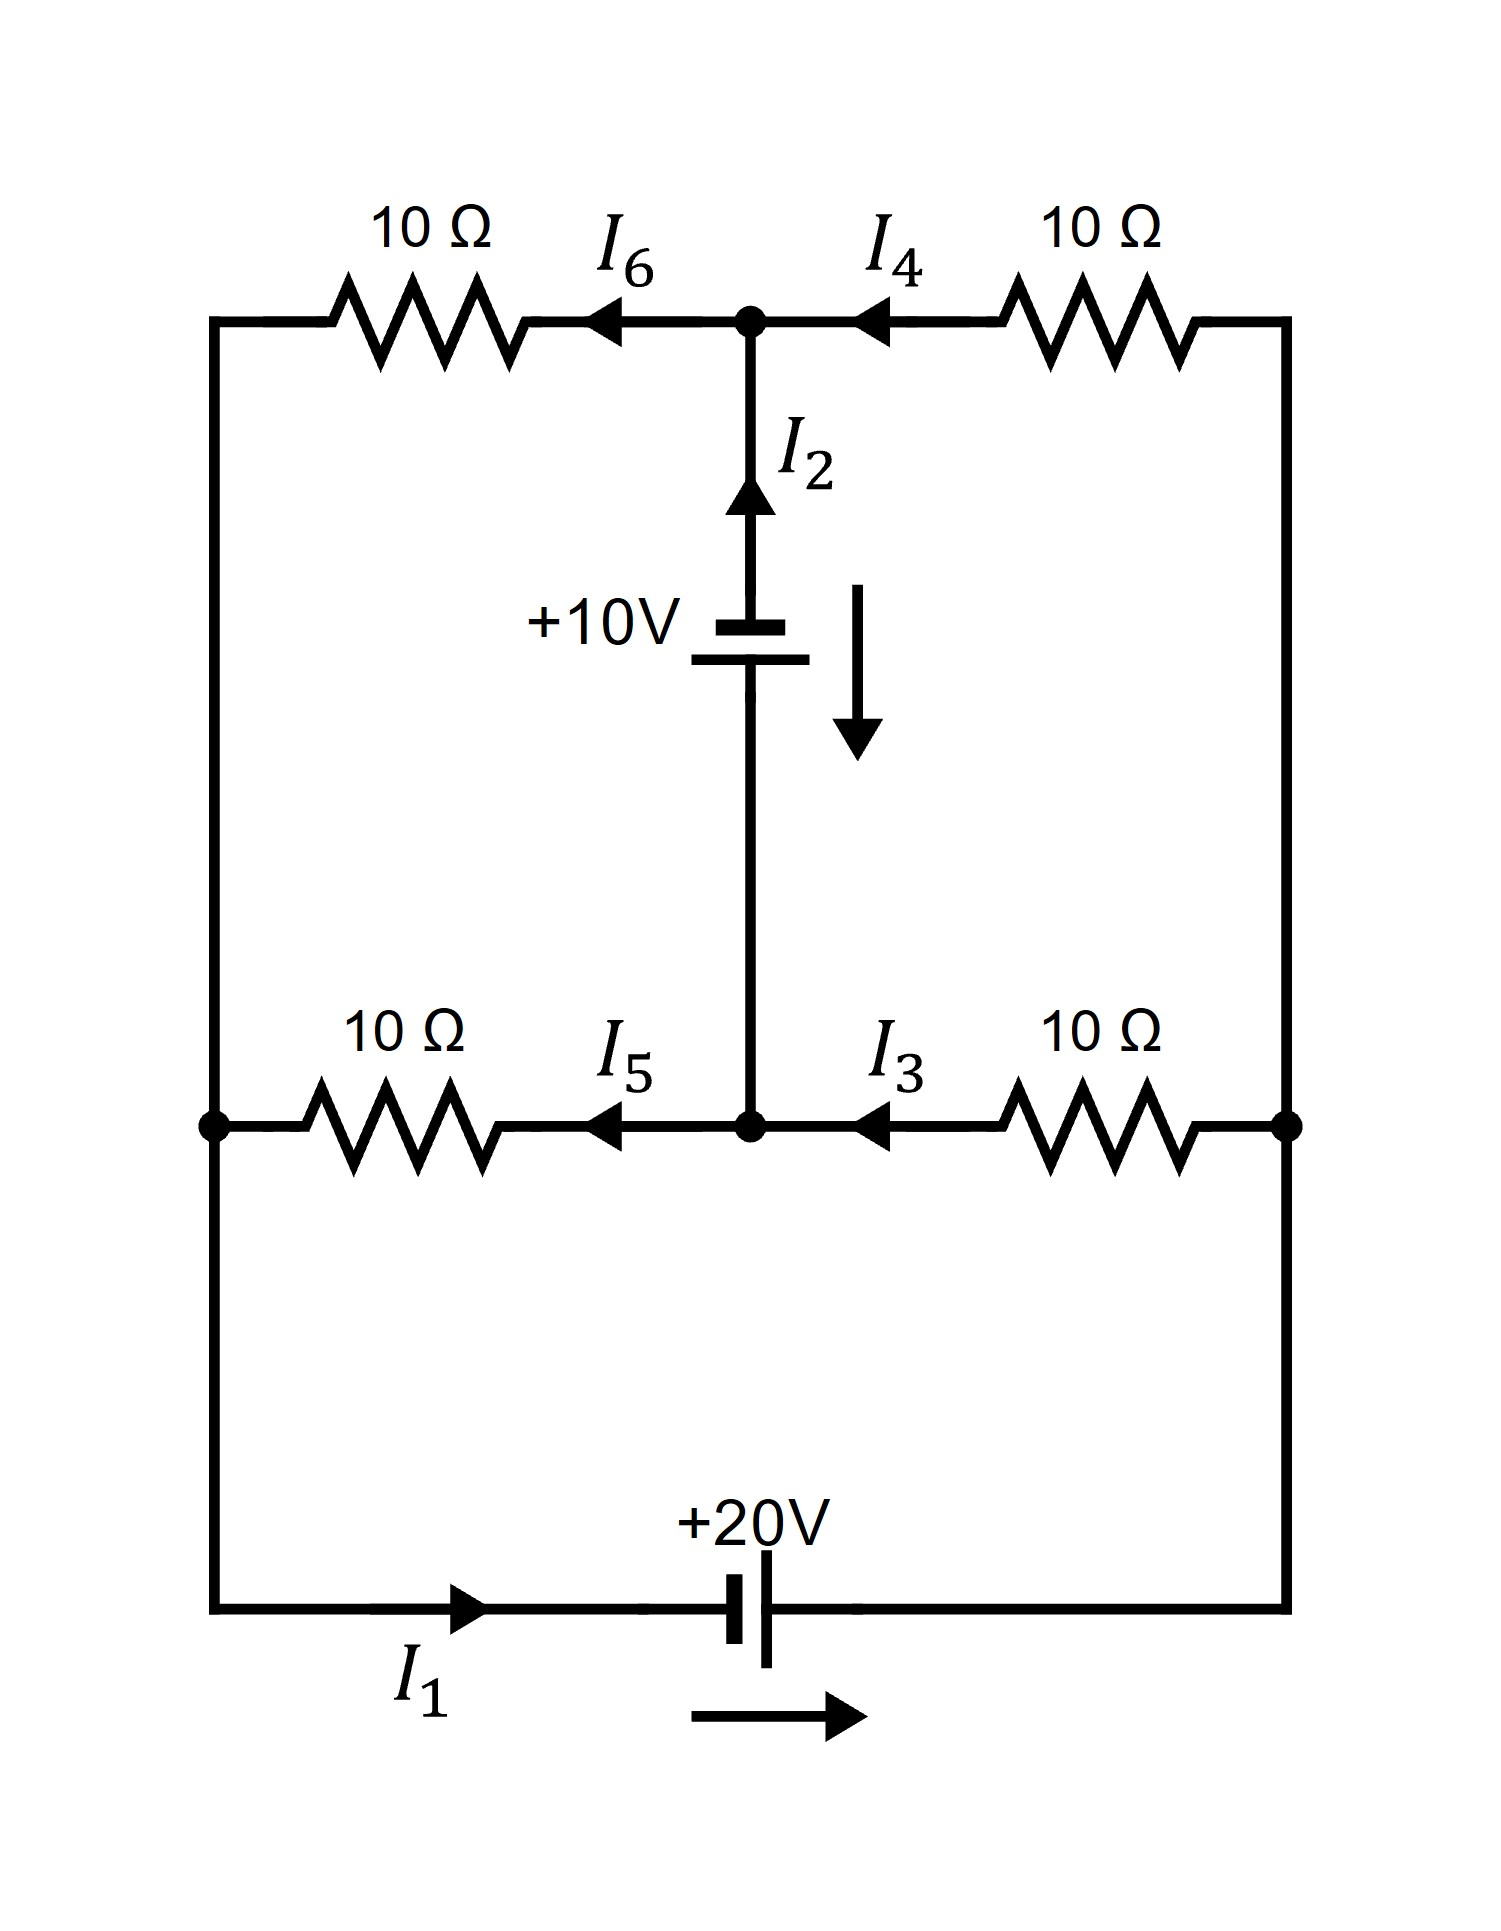
\includegraphics[height=1.2in]{circuit500.jpg}~
 
\end{image}

$ I_1 = \answer{2}$, $I_2 = \answer{1}$, $I_3 = \answer{\frac{1}{2}}$, $I_4 = \answer{\frac{3}{2}}$, $I_5 = \answer{\frac{3}{2}}$, $I_6 = \answer{\frac{1}{2}}$

\end{problem}

\begin{problem}\label{prob:circuit6}

Find the voltage $x$ such that the current $I_1 = 0$.

\begin{image}
   
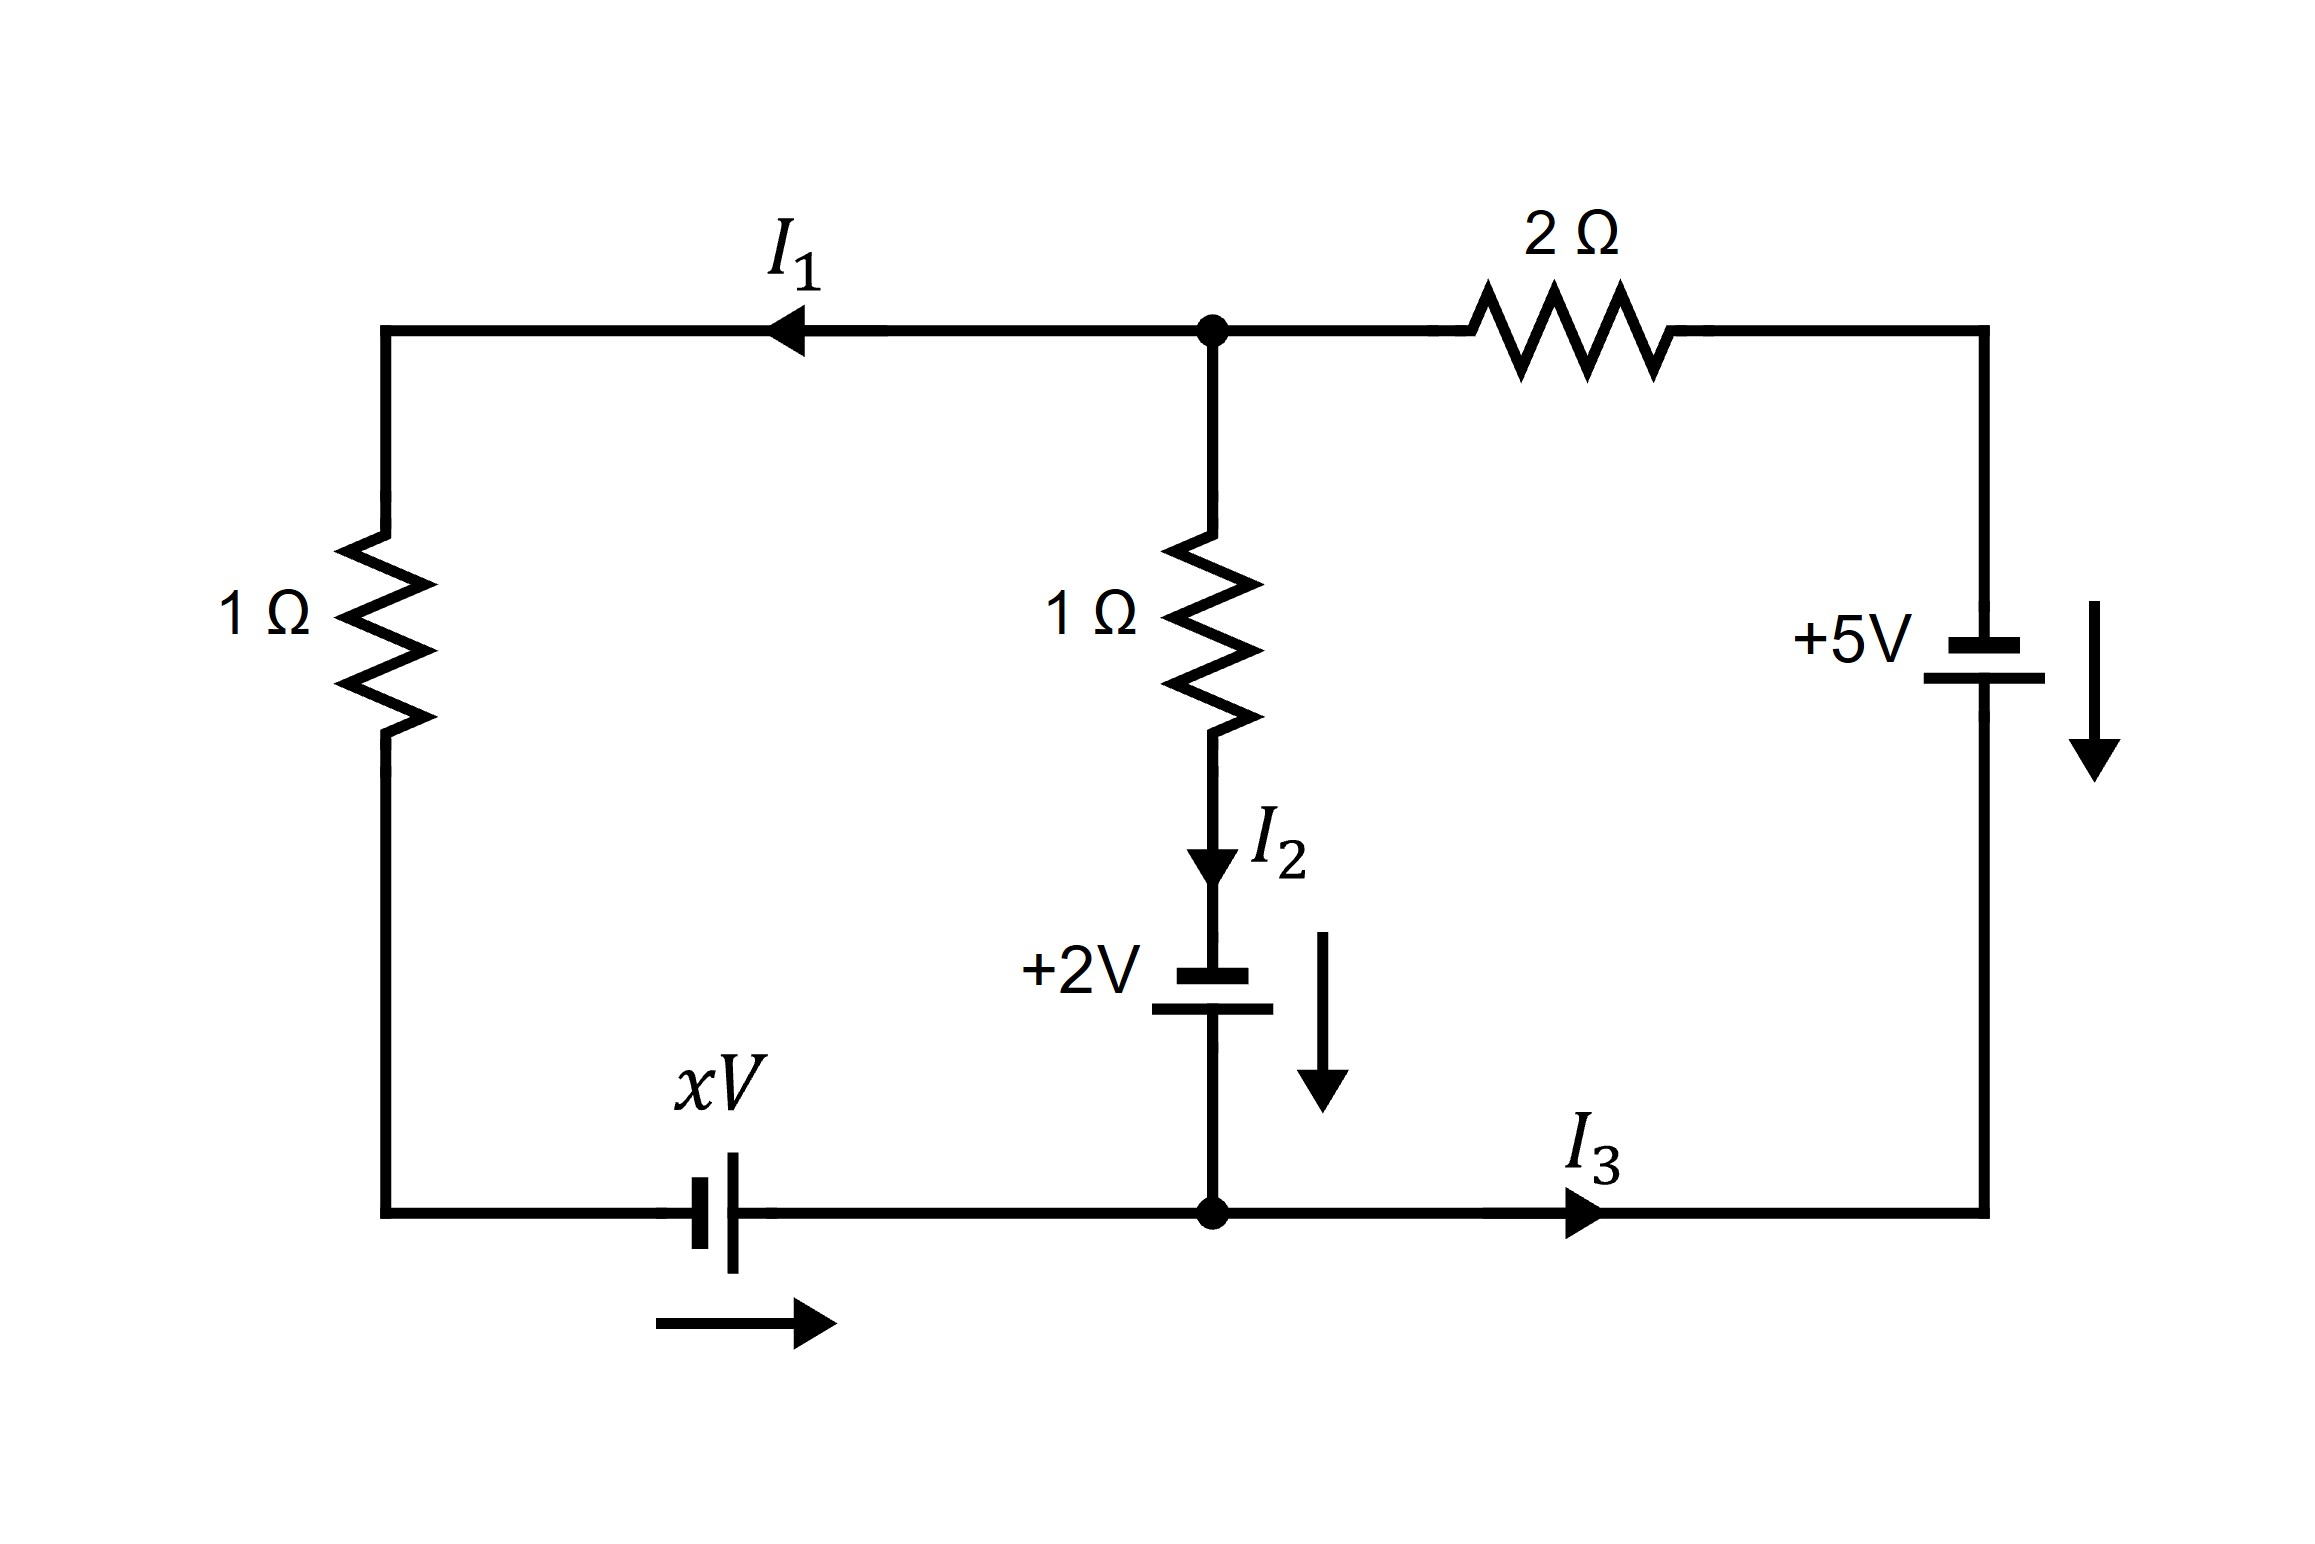
\includegraphics[height=1.2in]{circuit600.jpg}~
 
\end{image}

$x = \answer{1}$
\end{problem}

\section*{Text Source} This application was adapted from Section 1.5 of Keith Nicholson's \href{https://open.umn.edu/opentextbooks/textbooks/linear-algebra-with-applications}{\it Linear Algebra with Applications}. (CC-BY-NC-SA)

W. Keith Nicholson, {\it Linear Algebra with Applications}, Lyryx 2018, Open Edition, p. 29 

Circuit Diagrams were made using \href{https://www.circuit-diagram.org/}{\it https://www.circuit-diagram.org/}

\end{document}